
\section{Overview of the Silicon Tracking System}
\subsection{Role of the tracker}
\subsection{Silicon Sensors}
\label{sensors}
One of the important parameters of the silicon sensor is leakage current, which is strongly correlated with the temperature as per equation \ref{Sil:temp} \cite{Hartmann:2017gzy}.

\begin{equation}
\label{Sil:temp}
    I_{R}(T) \propto T^{2}e^{\frac{-E}{2kT}}
\end{equation}

 By assuming that one of the  temperature sensors at a similar height as the silicon sensors mimics their temperature. This assumption clearly doesn't consider several effects like silicon sensors' self-heating. Nevertheless, it allows us to scale down leakage current to $20\,^{\circ}$C using the equation \ref{Sil:scal}.
 
\begin{equation}
\label{Sil:scal}
    \frac{I_{R}(T_{2})}{I_{R}(T_{1})} = (\frac{T_{2}}{T_{1}})^{2}e^{\frac{-E}{2kT}\frac{T_{1}-T_{2}}{T_{1}T_{2}}}
\end{equation}

\begin{figure}[!h]
\centering
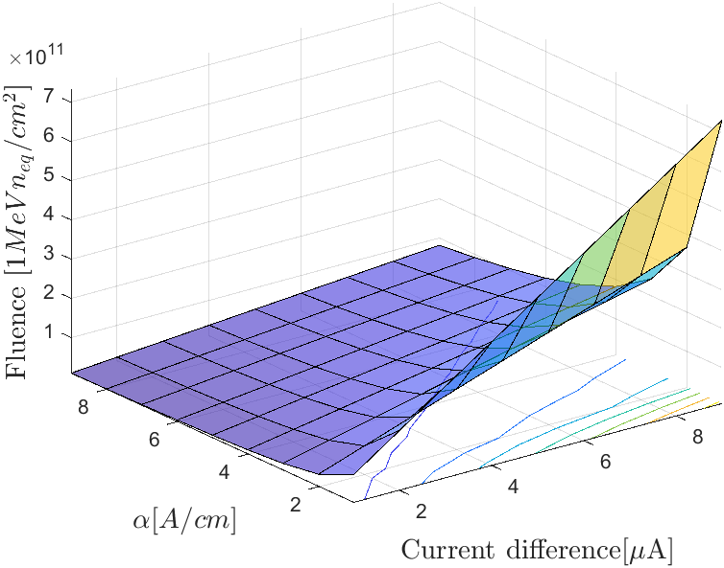
\includegraphics[width=0.65\columnwidth]{Chapter2/images/Leakage_current.png}
\caption{The first proposition of the CBM readout chain based on separate DPB and FLIB boards \cite{CRI}}
\label{fig_leakage}
\end{figure}

\begin{figure}[!h]
\centering
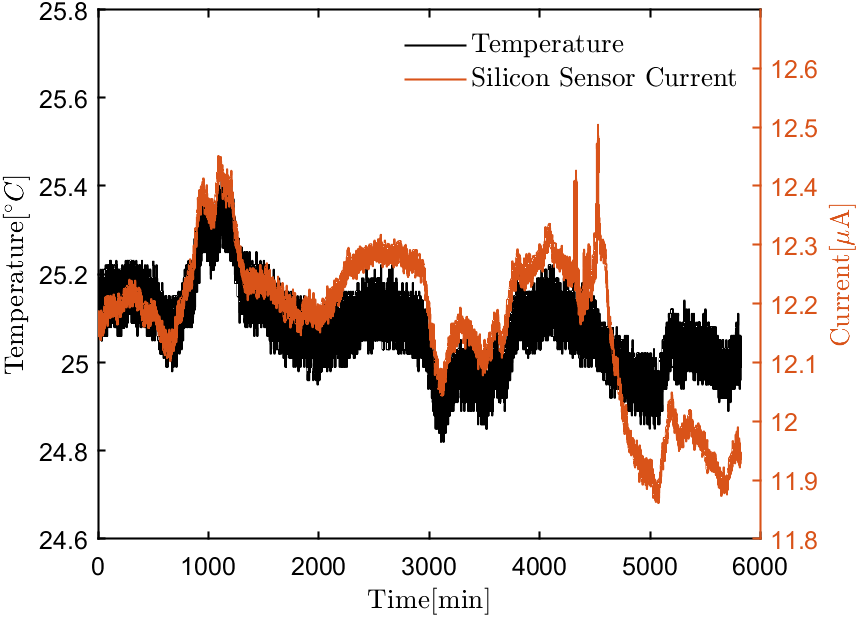
\includegraphics[width=0.65\columnwidth]{Chapter2/images/currenttempnobeam.png}
\caption{The first proposition of the CBM readout chain based on separate DPB and FLIB boards \cite{CRI}}
\label{fig_leakage1}
\end{figure}



\subsection{Module}
\subsection{STS-XYTER}
\subsection{Front End Boards}
\label{module}
\subsection{Readout chains}
\label{readout}
\label{DAQ}
There are three main readout chains that have been exercised for different detector development activities.  
The readout chain used in the module or FEBs test is built from two components: 
\begin{enumerate}
    \item the Common Readout Board (\gls{CROB}) for data concentration and transport with electrical to optical interface (see figure 
    \item Data Processing Board (DPB) based on the AFCK board (see Fig.
\end{enumerate}

\begin{figure}[!h]
\centering
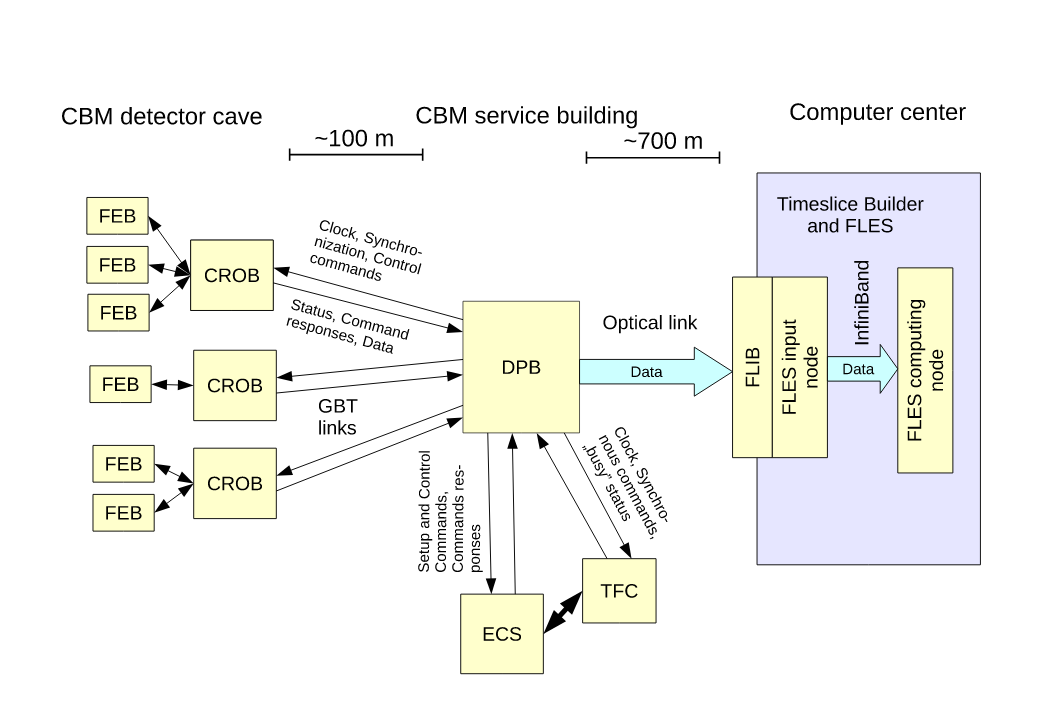
\includegraphics[width=0.65\columnwidth]{Chapter2/images/DPB.png}
\caption{The first proposition of the CBM readout chain based on separate DPB and FLIB boards \ref{fig_cri_board}}
\label{fig_dpb_scheme}
\end{figure}

\begin{figure}[!h]
\centering
\includegraphics[width=0.65\columnwidth]{Chapter2/images/feb_8_v2.pdf}
\caption{FEB}
\label{fig_febA_photo}
\end{figure}
\subsection{CRI based readout chain}
\begin{figure}[!h]
\centering
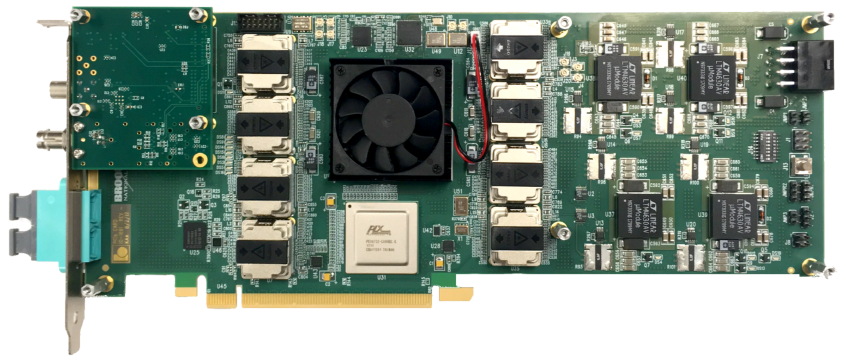
\includegraphics[width=0.65\columnwidth]{Chapter2/images/cri_board_atlas.pdf}
\caption{CRI board}
\label{fig_cri_board}
\end{figure}
\subsection{DPB based readout chain}

\subsection{Tester readout chain}
\label{tester}
Another alternative to the two readout chains introduced in the last two sections is so-called GBTxEMU-based tester. It is based on a commercial Artix-7 board (TE-0712, Trenz Electronics Gmbh), and allows emulating GBTX ASIC or the whole CROB. Moreover, it could also be used in an autonomous mode with the addition of VITA  57.1 FMC adapter

\subsection{Cooling}
\label{cooling}
\subsection{Powering scheme}
\label{powering}
\subsection{Detector enclosure}
\section{Requirements for the control system} 
Custom solutions which are applied in the \gls{STS} make the control of this system even more challenging. In fact, the control frameworks needs to be very broad to address that problem.
 The \gls{DCS} for the Silicon Tracking System (\gls{STS}) is being designed taking into consideration the following aspects:
 \begin{itemize}
     \item applications should be easy to run on different operating systems and processor architectures,
     \item horizontal and vertical scalability, when it comes to adding additional computing nodes or applications/Input Output Controllers (\glspl{IOC})/containers,
     \item it should be possible to integrate a sub-system oriented \gls{EPICS}-based \gls{DCS} with higher-level control structures,
     \item the system should be highly available, minimizing the downtimes,
     \item it should be running in a dedicated network (divided into several service-oriented subnets) to have a good overview of the processes and communication between the nodes,
     \item all parameters/\footnote{In control theory, a process variable is the current measured value of a particular part of a process which is being monitored or controlled}{process variables} should be available in a user-friendly Graphical User Interface (\gls{GUI}). In case of error or malfunction it should be stated clearly by the software where the error happened, what could be the potential risk and what actions need to be taken,
     \item the experiment is supposed to run for about 10 years, excluding the building and commissioning time. The control system should be sustainable and long-term support provided,
     \item there should be reliable means of supervision of processes, containers, and \glspl{IOC}.
 \end{itemize}


